%情報処理学会全国大会原稿テンプレート ver. 1.2

\documentclass[uplatex,twocolumn]{jsarticle}
\usepackage[top=30mm,bottom=25mm,left=20mm,right=20mm]{geometry}
\usepackage[T1]{fontenc}
\usepackage{txfonts}
\usepackage[expert,deluxe]{otf}
\usepackage[dvipdfmx,hiresbb]{graphicx}
\usepackage[dvipdfm]{hyperref}
\usepackage{pxjahyper}
\usepackage{multicol}
\usepackage{here}
\setlength{\columnsep}{7mm}

\title{\vspace{-10mm}Twitter発言の分析によるWebサービス障害の影響調査\footnotemark[0]}
\author{\large{岩瀬 翔\footnotemark[2]\qquad 矢吹 太朗}\\千葉工業大学 社会システム科学部 プロジェクトマネジメント学科\footnotemark[3]}
\date{}
\pagestyle{empty}
\begin{document}
\twocolumn[\maketitle]

\begingroup
\def\thefootnote{\fnsymbol{footnote}}
\footnotetext[0]{Investigation of the influence of failure of web service based on tweet analysis.}
\footnotetext[2]{Sho IWASE (\verb|s1442012ap@s.chibakoudai.jp|)}
\footnotetext[3]{Department of Project Management, Faculty of Social Systems Science, Chiba Institute of Technology.}
\endgroup

\section{序論}
複数のメンバが同時に開発を行うソフトウェア開発プロジェクトにおいて,Webサービスが使われることがある.例えば,チーム内でファイルのバージョンを管理する「GitHub」や,コミュニケーションを取るためのチャットツール「Slack」である.

これらのサービスの停止は,それを利用しているプロジェクトに大きな影響を与えると思われる.実際,2016年1月28日のGitHubの停止時や,2017年11月1日のSlackの停止時には,そのせいで仕事が進められなくなったというようなつぶやきが,Twitter上で複数観測された\cite{01}.

\section{目的}

Twitterの発言を収集するためのツールを開発し,それを用いてソフトウェア開発で利用されるWebサービスの停止が開発に与える影響を調査する.

\section{手法}

本研究は以下の2段階で行う.
\begin{enumerate}
 \item Twitterからツイートを収集するためのツールを開発する.
 \item サービスの停止から復旧までに投稿されたGitHubに対するツイート数と,どのくらいの時間で復旧が完了するのかを調べる.
\end{enumerate}

初めに,Twitterで投稿されているGitHubの障害発生に関するツイートをデータとして収集する.TwitterのAPIには,1週間以上前のツイートを検索して取得することができないという制限があるため,本研究のためには使えない\cite{02}.そこで,インターネットブラウザ上のTwitterで使用できる「高度な検索」を利用する.高度な検索は,APIによる検索で取得できない期間やいいね・リツイートの数で絞り込むなどといったことが可能になっている.さらに,検索結果を特定の期間や特定のユーザー・言語などに絞り込むことができ,探しているツイートも見つけやすくなる.本調査では「キーワード,言語,日時,期間」を指定して検索する.例えば,序論で述べた2016年1月28日に発生したGitHubの障害発生について検索する場合,「GitHub lang:ja since:2016-01-28\_00:00:00\_JST until:2016-01-29\_00:00:00\_JST」となる.検索結果はブラウザを最下部までスクロールすることで古いものが読み込まれていく.これを繰り返すことで,2016年1月28日に投稿された「GitHub」を含む日本語のツイートを全て表示できる.このブラウザを使ったTwitterの検索画面からツイートの本文と時間のみをWebスクレイピングするためのツールを開発し,過去のツイートを取得する.

ブラウザのTwitter検索結果からデータを収集するツールを開発するために2つのプログラムを作成する.1つ目のプログラムでは検索画面を最下部までスクロールする作業とページ全体をHTMLファイルで保存する作業を自動化する.ブラウザのスクロール作業を自動で行う必要があるため,ブラウザの自動操作ができるライブラリである「Selenium WebDriver」を使用し,検索結果をブラウザに全て表示させてからHTMLファイルで保存する.2つ目のプログラムでは,保存したHTMLファイルからツイートの本文と時間のみ抽出するため,Pythonのライブラリであり,HTMLファイルを解析してスクレイピングを行うことのできる「BeautifulSoup4」を使ってデータを抽出する.

データを取得する日を特定するため,GitHubに関連するすべてのサービスを継続的に状況監視している「GitHub Status」の「Status Message」を参照し,2016年で主要なサービスが停止,復旧したとアナウンスされている時間を調べる.その日のツイートを作成したツールを使って検索し,ツイートの時間と本文のみを抽出する.これを各障害の発生日ごとに実行する.

\section{結果}
GitHub StatusのStatus Messageを参照に調べたところ,2016年のGitHubにおけるサービス停止回数は14回であった(ただし,10月21日の障害は同時にTwitterにも障害が発生していたため,対象に加えていない).

% 大文字のHを使用することで好きな位置に図を配置
\begin{figure}[H]
%\includegraphics[width=図の幅,clip]{ファイル名}\label{参照用ラベル}
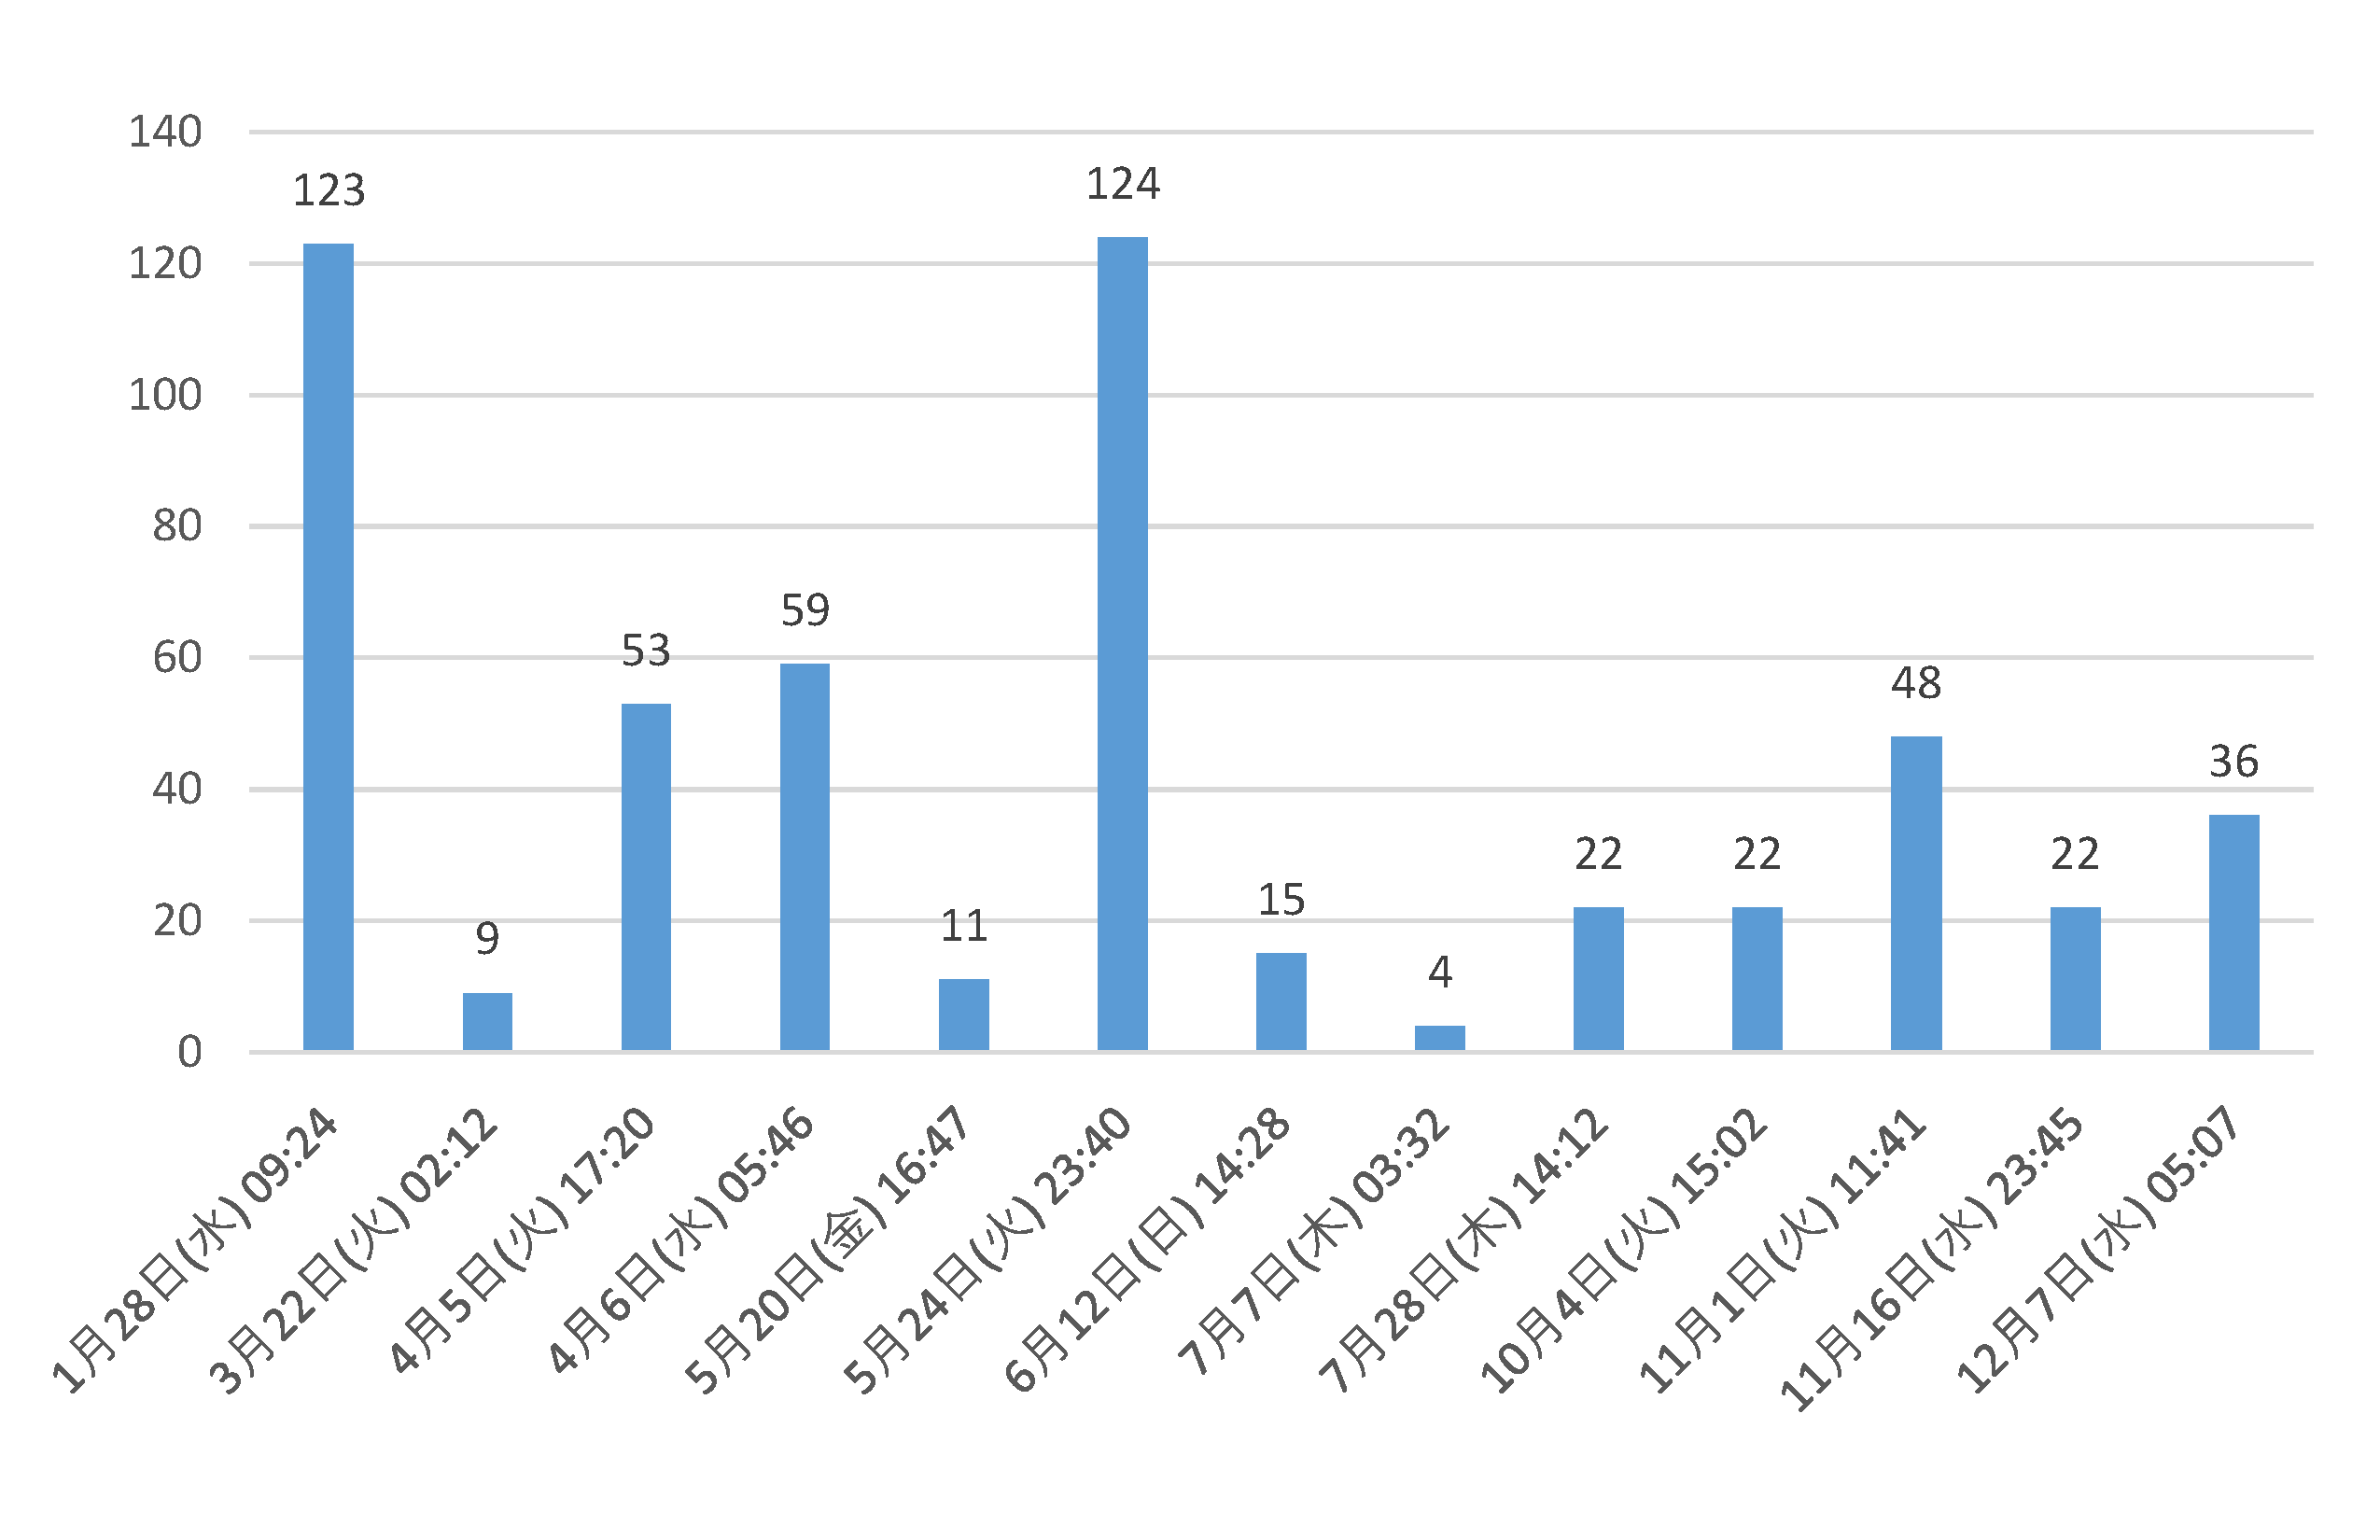
\includegraphics[width=7.6cm,clip]{graph1.pdf}
\caption{サービス停止から復旧までの間隔}\label{時間}
\end{figure}
\begin{figure}[H]
%\includegraphics[width=図の幅,clip]{ファイル名}\label{参照用ラベル}
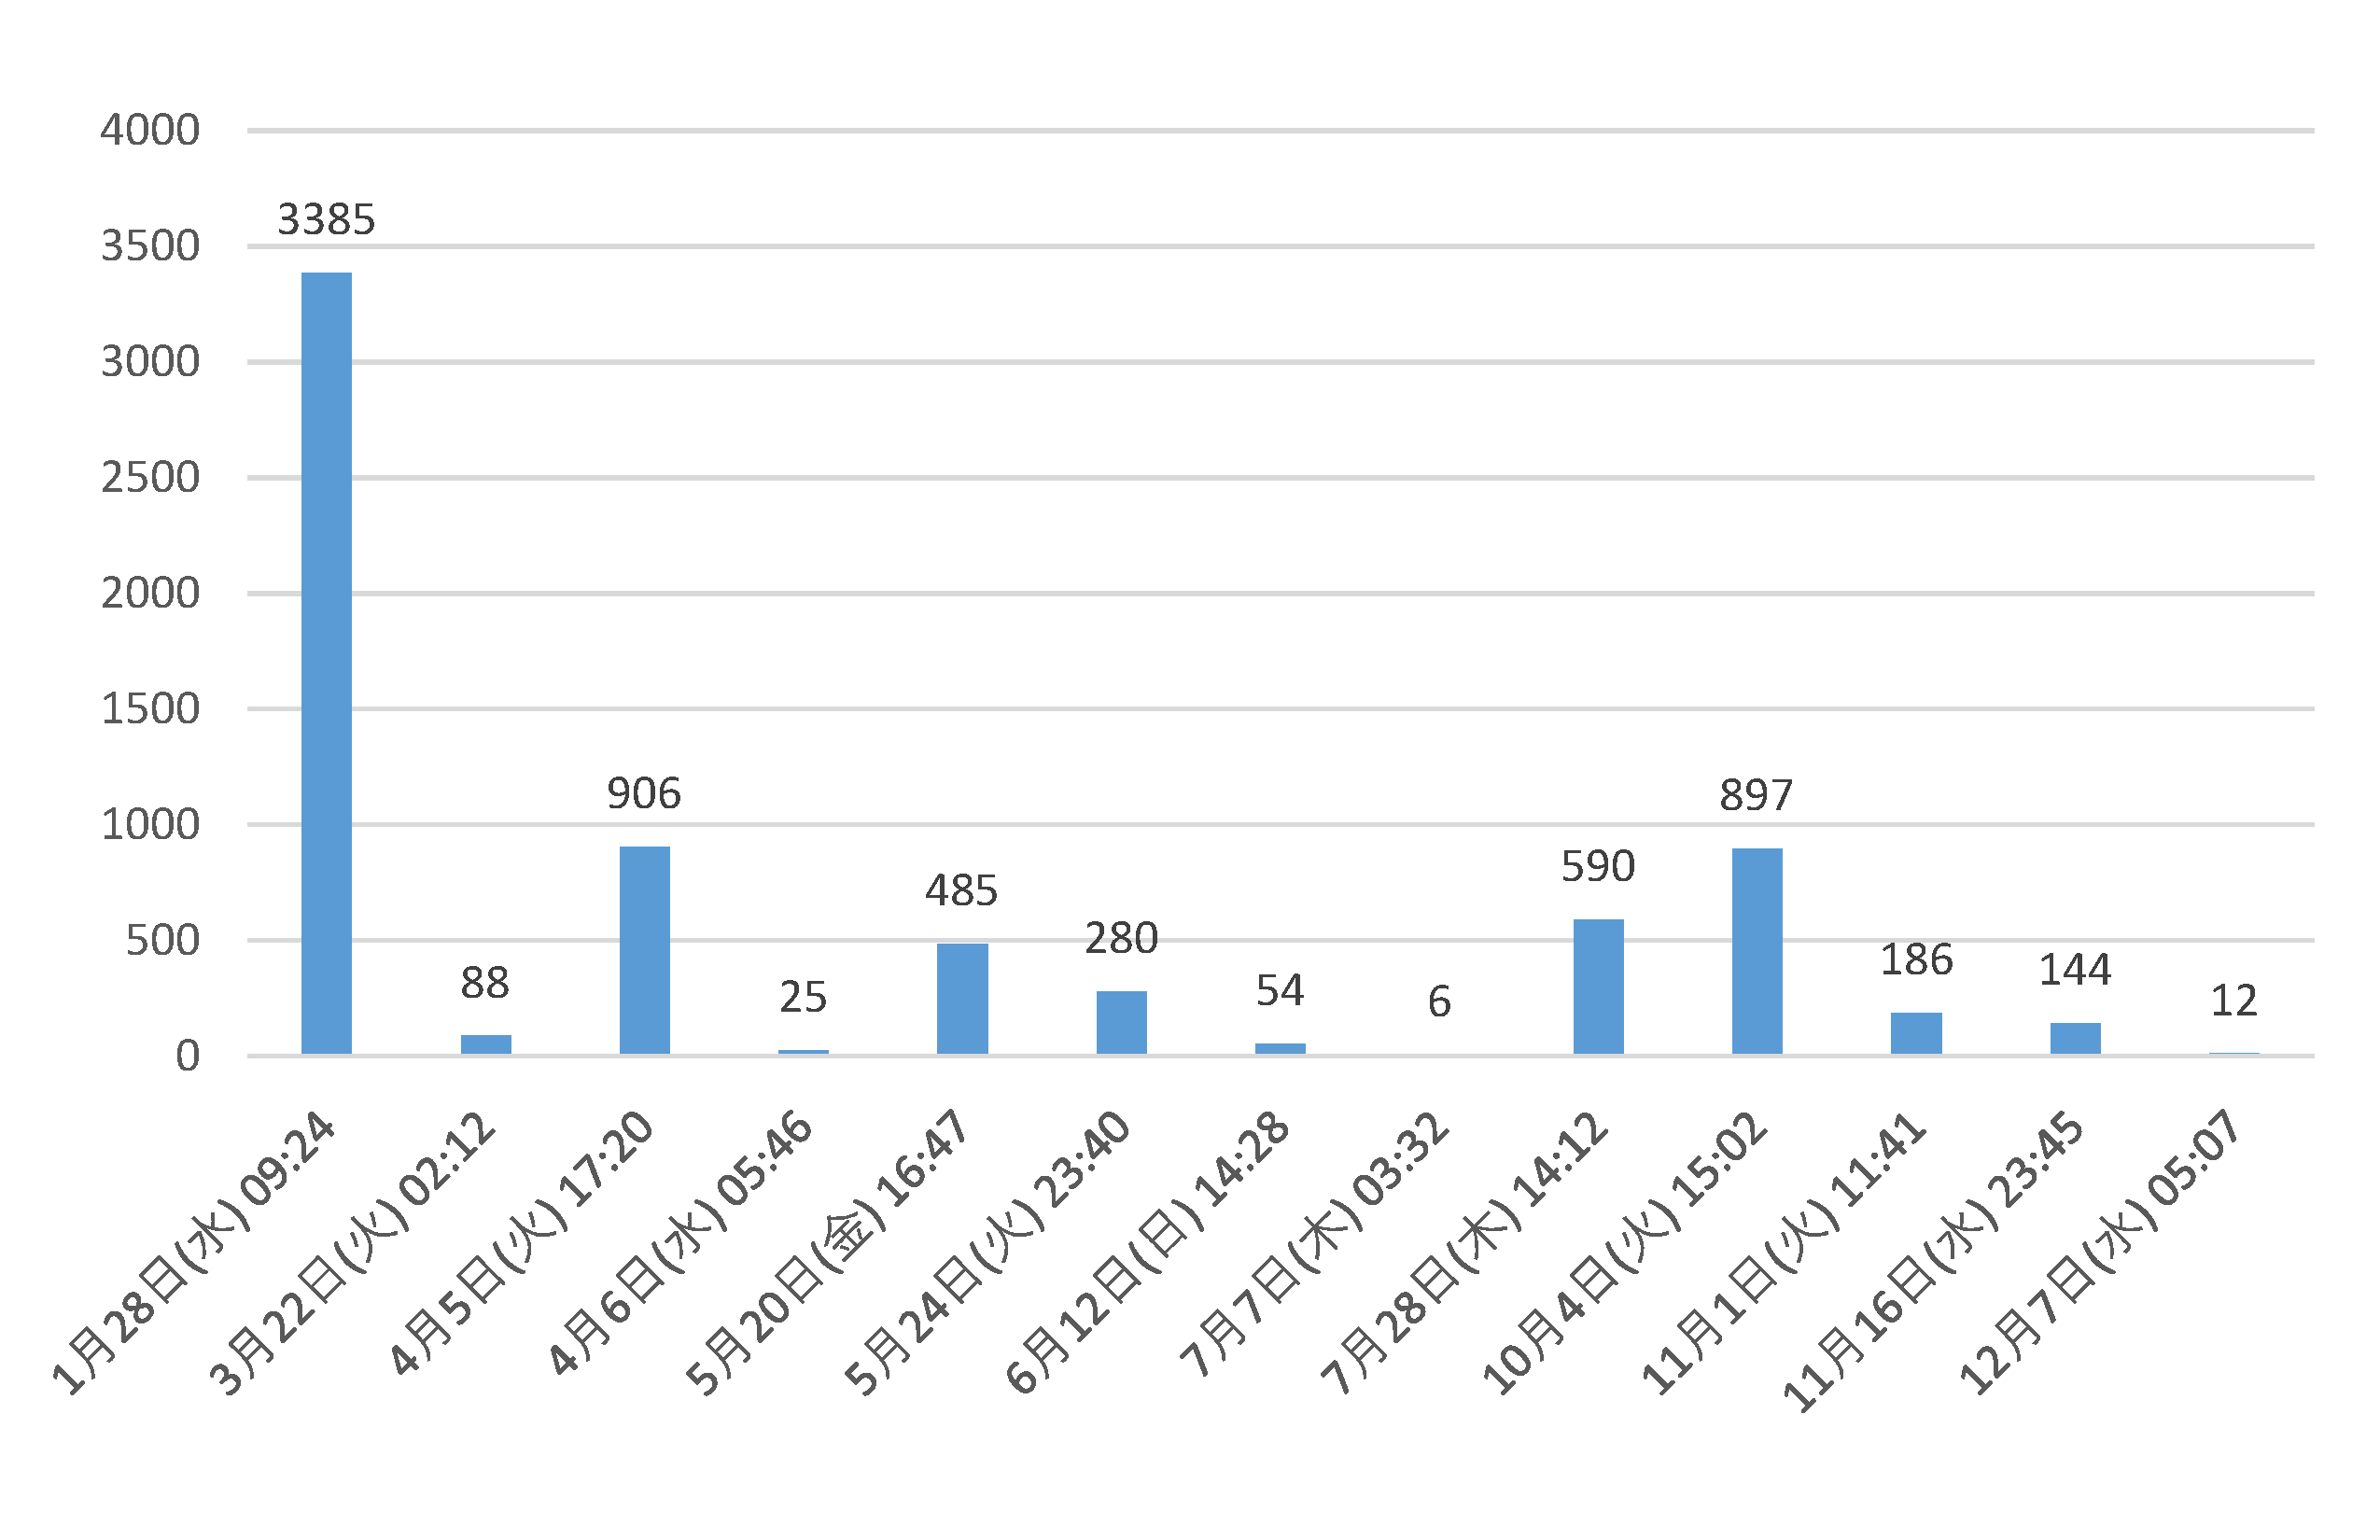
\includegraphics[width=7.6cm,clip]{graph2.pdf}
\caption{サービス停止中に投稿されたツイートの数}\label{ツイート数}
\end{figure}
13回分の各障害のサービス停止から復旧までの間隔を分単位でグラフにしたものが図\ref{時間}である.

そして,各障害のサービス停止中に投稿されたツイート数をグラフにしたものが図\ref{ツイート数}である.

\section{考察}
調査した13回分の障害を比較すると,サービス停止から復旧までの間隔が同じくらいでも,1日の時間帯によってツイート数に違いがあった.特にツイート数が多かったのは平日の日中で,中でも会社への出勤や退勤にあたる時間帯であった.この時間帯にWebサービスが停止してしまうと例え数分の停止でもツイート数が多く,1日のタスクが確認できなかったり,チーム内でのコミュニケーションが取れなかったりする.1月28日(水)が最も多い3385ツイートとなっているが,やはり9時台という出勤にあたる時間で2時間以上の停止をしたことが原因だと考える.日中の障害でも6月12日(日)と7月28日(木)では同じ14時台の障害で停止時間に約7分の差はあるが500ツイート以上の差があった.これは日曜日に起きた障害であり,普段仕事をしている人々が休暇中であったため少なかったと考える.

平日の日中であればツイート数が多いのはもちろんだが,3月22日(火)の深夜2時台に発生した約9分間の障害でも88件のツイートが集まった.この時間でも仕事にならないという反応が観測されている.

以上のことから,ソフトウェア開発プロジェクトなどでWebサービスを使用する場合は,サーバーダウン等の障害が発生するリスクを考慮する必要があることがわかる.

また,本研究ではGitHub StatusのStatus Messageを参照してツイート取得する日を決定していたが,Status Messageに記されているサービス停止や復旧のアナウンスよりも,サービスが停止・復旧したというツイートの方が平均約8分早く観測されていた.このことは,サービスの状態について運営元が発表している情報が必ずしも正しくはないことを示唆している.このことは,サービス停止がビジネスに重大な影響を及ぼす状況では,問題になり得る.

\section{結論}
Twitterのブラウザでの検索結果を保存するツールを開発し,それを用いてGitHubやSlackなどのウェブサービスの停止に対する開発者の反応を調査した.その結果,日中はもちろん深夜でもサービス停止の影響は大きいこと,サービス運営元による停止時間についての発表は実際のそれとはずれていることがわかった.このようなデータがあることから,ウェブサービスの停止を考慮したリスクマネジメントの実践が期待される.
\bibliographystyle{junsrt}
\bibliography{biblio}%「biblio.bib」というファイルが必要.


\end{document}